
\documentclass[conference]{IEEEtran}

\ifCLASSINFOpdf

\else

\fi

\setlength\parindent{0pt}
\onecolumn
\usepackage{textcomp}
\usepackage{amsmath}
\usepackage{float}
\usepackage{fancyvrb}
\usepackage{float}
\usepackage{graphicx}

\newenvironment{tightcenter}{%
  \setlength\topsep{0pt}
  \setlength\parskip{0pt}
  \begin{center}
}{%
  \end{center}
}

\begin{document}

\title{ELEN4020 Lab Two Report}


\author{\IEEEauthorblockN{Arlo Eardley (1108472), Carel Ross (1106684) and Ryan Verpoort (1136745)}
\IEEEauthorblockA{School of Electrical and Information Engineering, University of the Witwatersrand, Johannesburg 2050, South Africa}}

\maketitle

\IEEEpeerreviewmaketitle

\section{Overview}

The work conducted involves the use of Pthread and OpenMP written in the C programming language. The main function has an input for the value of N. This will determine the size of the two-dimensional array since N=N0=N1, where the array is declared as follows:\\

A[N0][N1]\\

The values assigned to each element in the array will be generated as follows:\\

A $<$i, j$>$ = i*N + j\\

Where i and j indicate the position of the element in the matrix.



\section{Memory Management}

Three specific sizes of N are tested. These values are 128, 1024 and 8192. The matrix is allocated as an array of integers, where each integer is 4 bytes. This design choice is flexible since an array of short floating points can also be used. This means that the total memory required for the array is as follows:\\

N^2*4\\

The total memory required for N = 128 is 65,536 bytes, N = 1024 is 4,194,304 bytes and N = 8192 is 268,435,456 bytes. These are relatively large amounts of memory that are required, therefore, the array is structured as shown in Figure 1. Figure 1 demonstrates an example where N = 4. This means that there is a pointer array of size N, where each element of this array points to a N size integer array.


\noindent
\begin{figure}[H]
\centering
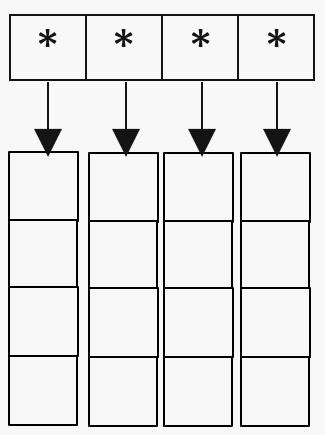
\includegraphics[scale = 0.5]{Figure1.png}
\caption{}
\end{figure}


The largest block of contiguous memory required would therefore be of size N. This will allow for larger values of N to be evaluated since there are multiple arrays distributed across memory. Since pointers are used, the pointers need to be freed and deleted to avoid memory leaks. \\


If the array were assigned to a standard two-dimensional array, then the amount of data that can be processed would be severely limited since one large block of contiguous memory would be required. For example, if in the case of an array that is 268 MB or larger, then you would be limited to where you can put the data, which may possibly even lead to it being placed in virtual memory, limiting the speed of computation. \\


\section{Transposition and Shared Memory}

The method of transposition used is demonstrated in Figure 2 and Figure 3. From a reference point the first blocks are switched, which required one operation in the loop, as shown in Figure 2. The second iteration will require two operations to transpose those particular elements. This continues until all operations have been completed, which will then result in a fully transposed matrix. By using shared memory, operations can be completed by multiple threads. This means that operations can be completed in a parallel manner, therefore increasing the speed of computation. \\

\noindent
\begin{figure}[H]
\centering
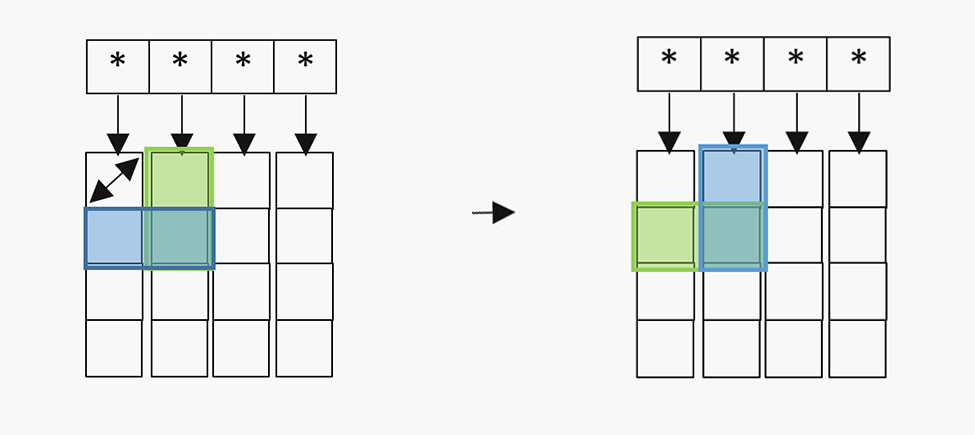
\includegraphics[scale= 0.4]{Figure2.png}
\caption{}
\end{figure}

\noindent
\begin{figure}[H]
\centering
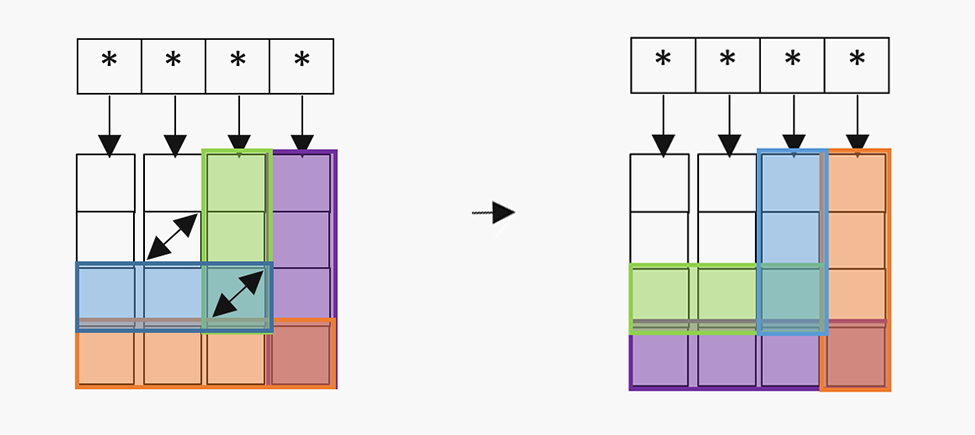
\includegraphics[scale= 0.4]{Figure3.png}
\caption{}
\end{figure}

The transposition solution looks at the matrix in three processes consisting of two nested for loops as follows:\\

\begin{enumerate}
\item The first process goes through the top left quadrant of the array.
\item The process goes through the bottom right quadrant of the array.
\item The third process goes through the remaining two quadrants.\\
\end{enumerate}

These tasks are illustrated below where the numbers correspond to the three aforementioned processes:\\


\[
\begin{bmatrix}
 \textbf{1} &\textbf{1} & \textbf{1} & 3 & 3 & 3 \\
 \textbf{1} & \textbf{1} & \textbf{1} & 3 & 3 & 3  \\
 \textbf{1} & \textbf{1} & \textbf{1} & 3 & 3 & 3 \\
 3 & 3 & 3 & \textbf{2} & \textbf{2} & \textbf{2} \\
 3 & 3 & 3 & \textbf{2} & \textbf{2} & \textbf{2} \\
 3 & 3 & 3 & \textbf{2} & \textbf{2} & \textbf{2} \\

\end{bmatrix}
\]

\bigskip

\section{OpenMP}

The omp parallel directive is used to indicate to the compiler that the block of code within its scope is to be run in parallel. By using the shared keyword, it indicates that all values within the parameters, will be shared by all threads, these parameters include the size of the array (N), the array itself (A) and the size of the chunk used, in this case the size of the chunk is the integer 4. By using the private keyword, it indicates that all values within the parameters are to be private to each thread, these parameters include the iterator i, j and the temporary integer value used for swapping the values in the array.\\

The omp for directive is used to split the iterations of the loop across the various threads. These threads have already been initialized to work in parallel, therefore the various iterations of the loop will be run in parallel. By using the dynamic keyword, it indicates that all iterations of a loop are dynamically split into chunks that are run on various threads, this process continues until the loop is complete. By using the nowait keyword each thread continues without waiting for other threads to finish before starting the next operation.\\


\section{Pthreads}

There will be an array of threads created. These threads will be started using the pthread\_create() function. All the threads that are started will call the Transpose function. This means that each thread will be allocated a different task within the Transpose function. Another argument is also used as a parameter in the pthread\_create() function to isolate the various tasks conducted by each thread. This manually splits up the work done by each thread and is determined within the Transpose function. The pthread\_join() function is then called for each thread. This combines all the work done by each individual thread. This will parallelize the computation. \\


\section{Results}

\noindent Naive indicates an approach without threading. The values for N that are tested are 128, 1024, 8192\\

\begin{table}[H]
\centering
\caption{A table of Results for the transposition algorithm} 
\begin{tabular}{|c|c|c|c|c|}
  \hline
 Approach & Number of threads & N0=N1=128 (s) & N0=N1=1024 (s) & N0=N1=8192 (s) \\
\hline

Naïve	&   1	& 0.000230	  & 0.017072    &   3.691947\\
\hline
Pthread	&   4	& 0.000670	  & 0.009538    &   1.640811\\
\hline
OpenMP	&   4	& 0.000872    & 0.025300    &  	1.630964\\ 
\hline
Pthread	&   8	& 0.001011	  & 0.013418    &	1.743164\\
\hline
OpenMP	&   8	& 0.000872    & 0.027636    &  	1.737098\\
\hline
Pthread	&   16  & 0.003531	  & 0.019625	&   1.761639\\
\hline
OpenMP	&   16  & 0.001639    & 0.030240    &  	1.755257\\
\hline
Pthread	&   64  & 0.009504	  & 0.033195    &	2.105213\\
\hline
OpenMP	&   64  & 0.004855    & 0.032764    &  	1.771527\\
\hline
Pthread	&   128 & 0.011268    &	0.035964    &  	2.141281\\  
\hline
OpenMP	&   128 & 0.010520    & 0.034253    & 	1.816840\\

\hline
\end{tabular}

\end{table} 

When the array is relatively small, then the fastest method is the naive approach. This is due to the naive approach not requiring to allocate work to various threads, which takes time. Pthread consistently computes faster than the naive approach and OpenMP when N is 1024. This is due to Pthread allowing fast access to the threads. The optimal number of threads from the tested set is four. Finally OpenMP is optimal for very large arrays since the compiler can decide how each thread should allocate its work. Again the number of threads that yield the best results is four. This is due to the access time and work allocation for a large number of threads taking time, as well as the physical limitation of 4 threads. This means that any other threads will become virtual, severely decreasing computation speed. The system is scalable due to the format of memory management, as well as the structure of the threads.\\

\newpage
\section{Pseudo-code pthreads}

\begin{Verbatim}

for N indices of A
    Allocate memory for N 1D arrays 
    for N-1 values
        Set index values secondary 1D arrays

Create Transpose Function
     for N / 2 - 1 values
        check if value has been done by another thread if not continue
            for N / 2 values
                     Mirror indices in top left quadrant about main diagonal

    for N / 2 - 1 values
        check if value has been done by another thread if not continue
            for N values 
                Mirror indices in bottom right quadrant about main diagonal

     for N / 2 values
        check if value has been done by another thread if not continue
            for N / 2 values 
                Mirror indices in bottom left and top right quadrants about main diagonal
End Function

Start timer

For N threads
    assign thread[i] to the value i
    create a new thread which then performs the transposition function
end for loop

For N threads
    Join the existing threads back into a single thread
end for loop

End timer

for N values    
    Unallocate the memory in matrix A

\end{Verbatim}



\newpage
\section{Pseudo-code openMP}

\begin{Verbatim}
Declare 1D pointer array A of size N

for N indices of A
    Allocate memory for N 1D arrays 
		for N-1 values
		    Set index values secondary 1D arrays	

Set number of threads
Start timing

	Start parallel section
	{
		Schedule parallel for loops
		{
		    for  i = 0 to i = N / 2 - 1 values
			    for i + 1 to i < N / 2 values
			         Mirror indices in top left 
			         quadrant about main diagonal
	         }
        }
        
	Start parallel section
	{
		Schedule parallel for loops
		{
		    for  i = N / 2  to  i = N - 1 values
			    for i + 1 to i < N values 
				    Mirror indices in bottom 
				    right quadrant about main diagonal
		}
	}
	
	Start parallel section
	{
		Schedule parallel for loops
		{
		    for i = N / 2 to i < N values 
			    for N / 2 values 
				Mirror indices in bottom left and
				top right quadrants about main diagonal
		}
	}
	
Stop timer
for N values	
	Unallocate memory in matrix A
    
Print out the time elapsed

\end{Verbatim}  



\end{document}



